%!TeX program = pdflatex
% Thomas Eskridge's Curriculum Vitae based on Geoff Boeing's 
% Email: teskridge@fit.edu
% Web: https://thomaseskridge.com/
% Repo: https://github.com/tce/cv

\documentclass[12pt,letterpaper]{report}

\usepackage[T1]{fontenc} % output T1 font encoding (8-bit) for accented characters as single glyph
\usepackage[strict,autostyle]{csquotes} % smart and nestable quote marks
\usepackage[USenglish]{babel} % regionalize hyphens, quote marks, etc automatically
\usepackage{microtype}% improve text appearance with kerning, etc
\usepackage{datetime} % enable formatting of date output
\usepackage{tabto}    % make nice tabbing
\usepackage{hyperref} % enable hyperlinks and pdf metadata
\usepackage{geometry} % manually set page margins
\usepackage{enumitem} % enumerate with [resume] option
\usepackage{titlesec} % allow custom section fonts
\usepackage{setspace} % custom line spacing
\usepackage{multicol}
\usepackage{multirow}

\usepackage[backend=biber, maxnames=99, giveninits=true]{biblatex}
\usepackage{graphicx}
\usepackage{booktabs}
\usepackage{pdfpages}

% Language setting
% Replace `english' with e.g. `spanish' to change the document language
%\usepackage[english]{babel}

% Set page size and margins
% Replace `letterpaper' with `a4paper' for UK/EU standard size
%\usepackage[letterpaper,top=2cm,bottom=2cm,left=3cm,right=3cm,marginparwidth=1.75cm]{geometry}

% Useful packages
\usepackage{amsmath}
\usepackage{wrapfig}
%\usepackage[backend=biber, maxnames=99, giveninits=true]{biblatex}
%\usepackage{graphicx}
%\usepackage{booktabs}
%\usepackage{pdfpages}



\defbibenvironment{myPublicationListYearStyle}
  {\list
     {\iffieldequals{year}{\bibyear}
        {}
        {\printfield{year}\savefield{year}{\bibyear}}}
     {\setlength{\labelwidth}{2em}%
      \setlength{\leftmargin}{\labelwidth}%
      \setlength{\labelsep}{\biblabelsep}%
      \setlength{\itemsep}{\bibitemsep}%
      \leftmargin\labelwidth%
      \advance\leftmargin\labelsep}%
   \renewcommand*{\makelabel}[1]{\hss##1}}%
  {\endlist}
  {\item}


\addbibresource{papers.bib}

\bibliography{papers.bib}

\nocite{*}

\defbibfilter{papers}{
  type=article or
  type=inproceedings
}


% what is your name?
\newcommand{\myname}{Thomas C Eskridge}

% select default typefaces
\usepackage{ebgaramond} % document's serif typeface
\usepackage{helvet}     % document's sans serif typeface

% how far to tab for list items with left-aligned date: different fonts need different widths
\newcommand{\listtabwidth}{1.7cm}

% define font to use as document's title
\newcommand{\namefont}[1]{{\normalfont\bfseries\Huge{#1}}}

% set section heading fonts and before/after spacing
\SetTracking{encoding=*, family=\sfdefault}{30} % increase sans serif headings tracking
\titleformat{\section}{\lsstyle\sffamily\small\bfseries\uppercase}{}{}{}{}
\titlespacing{\section}{0pt}{30pt plus 4pt minus 4pt}{8pt plus 2pt minus 2pt}

% set subsection heading fonts and before/after spacing
\titleformat{\subsection}{\lsstyle\sffamily\footnotesize\bfseries}{}{}{}{}
\titlespacing{\subsection}{0pt}{16pt plus 4pt minus 4pt}{4pt plus 2pt minus 2pt}

% set page margins (assumes letter paper)
\geometry{body={6.5in, 9.0in},
    left=1.0in,
    top=1.0in}

% prevent paragraph indentation
\setlength\parindent{0em}

% set line spacing
\setstretch{0.9}

% define space between list items
\newcommand{\listitemspace}{0.25em}

% make unordered lists without bullets and use compact spacing
\renewenvironment{itemize}
{\begin{list}{}{\setlength{\leftmargin}{0em}
                \setlength{\parskip}{0em}
                \setlength{\itemsep}{\listitemspace}
                \setlength{\parsep}{\listitemspace}}}
{\end{list}}

% make tabbed lists so content is left-aligned next to years
\TabPositions{\listtabwidth}
\newlist{tablist}{description}{3}
\setlist[tablist]{leftmargin=\listtabwidth,
    labelindent=0em,
    topsep=0em,
    partopsep=0em,
    itemsep=\listitemspace,
    parsep=\listitemspace,
    font=\normalfont}

% print only the month and year when using \today
\newdateformat{monthyeardate}{\monthname[\THEMONTH] \THEYEAR}

% define hyperlink appearance and metadata for pdf properties
\hypersetup{
    colorlinks  = true,
    urlcolor    = black,
    citecolor   = black,
    linkcolor   = black,
    pdfauthor   = {\myname},
    pdfkeywords = {city planning, housing, street networks, transportation, urban design, urban informatics},
    pdftitle    = {\myname: Curriculum Vitae},
    pdfsubject  = {Curriculum Vitae},
    pdfpagemode = UseNone
}

\begin{document}

    \raggedright{}

\begin{tabular}{ c l }
  \multirow{6}{*}{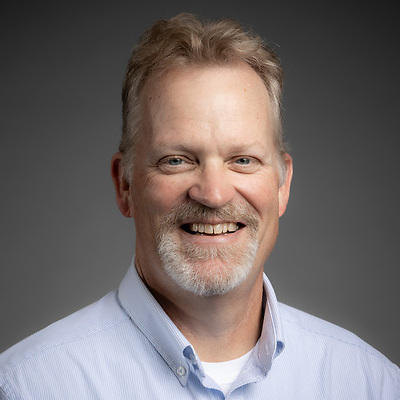
\includegraphics[height=1.75in]{img/headshot.jpeg}} & \large Thomas C Eskridge \\\\
  & \large teskridge@fit.edu \\
  & \large Harris Institute 311 \\
  & \large (321) 674-7455 \\
  & \vspace{20mm}\\
\end{tabular}


\subsection*{Brief History of the Candidate}

Dr. Thomas C Eskridge is a tenured Associate Professor in the Department of Electrical Engineering and Computer Science at Florida Institute of Technology (Florida Tech).  He arrived at Florida Tech as a Research Associate Professor in the L3Harris Institute for Assured Information, where he was Technical Lead or Key Personnel on a variety of projects sponsored by the Office of Naval Research, the Air Force Research Laboratory, the Department of Defense, as well as with large and small private companies.  Dr. Eskridge transitioned from a Research Associate Professor to Associate Professor and currently maintains an active research and teaching schedule focusing on techniques and processes that amplify human performance through teamwork with artificial intelligence (AI) agents and other automation.  Prior to joining Florida Tech, he was a Research Scientist at the Florida Institute for Human and Machine Cognition (IHMC) in Pensacola, FL.  There, he studied how visualizations can increase safety critical operator performance in aircraft and high-performance vehicles and how they can clarify operator knowledge for elicitation and instruction.  

Dr. Eskridge has been the principal investigator (PI) over \$300K of externally funded projects and has made contributions as Technical Lead (TL), Key Personnel (KP), or Contributor (C) on research projects totaling \$10,948,298.00.   He has published over 90 technical publications in scientific peer-reviewed conference proceedings such as \textit{ACM CHI Conference on Human Factors in Computing Systems}, \textit{International Conference on Case-based Reasoning}, \textit{International Conference on Applied Human Factors and Ergonomics}, and in peer-reviewed journals including \textit{New Space Journal}, \textit{IEEE Systems Journal}, \textit{EURASIP Journal on Information Security}, \textit{American Intelligence Journal}, \textit{IEEE Intelligent Systems}, \textit{Metaphor and Symbol}, and \textit{Journal of Information and Knowledge Management}. Before joining Florida Tech, Dr. Eskridge conducted research in Human-Centered Computing focusing on the development and commercial transfer of an aircraft instrumentation system that drastically reduced pilot instrument scan time and dramatically increased flying performance.  Dr. Eskridge is also an entrepreneur who founded a commercial visual inspection system company based on the similarity-based reasoning and learning system he developed as part of his Ph.D. dissertation.  This company, Intelligent Reasoning Systems, Inc., operated independently for ten years, with over 150 employees in offices around the world, including Taipei, Tokyo, London, and Frankfurt.  The combination of advanced research focused on practical applications throughout his career has resulted in 18 issued patents with Dr. Eskridge as inventor. 

\subsection*{Teaching and Related Activities}
\label{teaching}

My teaching contributions have been made primarily at the graduate level and have resulted in the development of eleven courses (see Table ~\ref{newcourse}).  Four of these courses were created as a result of the redesign of the Human-Centered Design degree program, an effort that I led for the department.  The driving goal for all of my courses is to put the topic in a practical, applied context so that students can use their hands-on projects as a tool to understand the science.  I also place a high value on working individually with students to help them understand how to conduct work and research in the topic or to make progress their degree program.  This commitment is evidenced by the consistent development of independent study courses that customize course content to address the topics that students are most excited and motivated to learn (see Table~\ref{indep}).   It is also evidenced by my commitment to students in the Capstone (see Table ~\ref{capstone}) and the undergraduate Senior Design classes (see Table ~\ref{srdesign}).  It is my belief that providing some extra attention to student interests and needs can instill in them a deeper appreciation for the subject and a significantly greater understanding of how to conduct research or development projects in an effective and efficient manner.   I believe that students will be able to leverage this understanding to increase their chances of success in their transition to industry or in the furtherance of the academic careers.  Students have responded to this approach by judging my teaching with an average evaluation for the semesters from 2017-2023 of \textbf{4.57}.  A detailed course description is shown in Table ~\ref{details} and a summary of evaluation scores is shown in Table~\ref{tabeval}.

\begin{table}
\caption{New Course Developments}
\label{newcourse}
\center
\begin{tabular}{| l | c | c | c | c | c | p{1.5in} |}
Num & Title & Required & Rec & Notes \\ \hline
HCD5210 & Introduction to Human-Centered Design & HCD & CSE/CYB & with GA Troy Weekes \\
HCD6380 & Creative and Design Thinking & HCD & No & with GA Troy Weekes \\
HCD5802 & Usability Engineering & HCD & No & \\
HCD6701 & Research Methods & HCD & No & \\
CSE5800 & Interacting with Large Language Models & No & CYB/CSE & \\
CYB5800 & Information Visualization & No & CSE/HCD & \\
CSE5800 & Deep Learning & No & CSE  & \\
CSE5290 & Introduction to Artificial Intelligence & No & CSE & \\
CSE5310 & Management and Processing of Big Data & No & CSE & \\
CYB5800 & Network Security Reasoning & No & CSE & \\
CYB5675 & Data Mining for Cybersecurity & No  & CSE/BISK & \\
\end{tabular}
\end{table}

\begin{table}
\caption{Detailed Course Descriptions}
\label{details}
\center
\begin{tabular}{| l | c | c | c | c | c | c |}
Semester & Title & Required & Rec & Enroll & Eval \\ \hline
Fall 2023 & Data mining for cybersecurity & No & Bisk CYB  & 2 & n.a. \\
Fall 2023 & Introduction to HCD & HCD & CYB/CSE  & 6 & n.a. \\
Fall 2023 & Interacting with LLMs & No & CSE  & 6 & n.a. \\
Spring 2023 & Usability & HCD & No  & 8 & 4.67 \\
Spring 2023 & Information Visualization & No & CSE  & 10 & 5.00 \\
Fall 2022 & Introduction to HCD & HCD & CYB/CSE  & 6 & 5.00 \\
Summer 2022 & Data mining for cybersecurity & No & Bisk CYB  & 4 & -- \\
Spring 2022 & Usability & HCD & No  & 8 & 5.00 \\
Spring 2022 & Research Methods & HCD & No  & 8 & 5.00 \\
Fall 2021 & Introduction to HCD & HCD & CYB/CSE  & 6 & 5.00 \\
Fall 2021 & Data mining for cybersecurity & No & Bisk CYB  & 9 & -- \\
Spring 2021 & Research Methods & HCD & No  & 8 & 5.00 \\
Fall 2020 & Usability & HCD & No   & 7 & 5.00 \\
Spring 2020 & Information Visualization & No & CSE  & 10 & 4.67 \\
Fall 2019 & Introduction to HCD & HCD & CYB/CSE  & 8 & 4.50 \\
Fall 2019 & Deep Learning & No & CSE & 12 & 4.67 \\ 
Summer 2019 & Data mining for Cybersecurity & No & NG CYB  & 6 & 4.00 \\
Fall 2018 & Artificial Intelligence & CSE & No  &  23 & 4.50 \\
Spring 2019 & Information Visualization & No & CSE  & 10 & 4.60 \\
Spring 2018 & Information Visualization & No & CSE  & 10 & 4.56 \\
Fall 2017 & Processing and management of big data & No & CSE & 16 & 4.67 \\
Spring 2017 & Information Visualization & No & CSE  & 10 & 5.00 \\
Fall 2016 &  Data mining for Cybersecurity & No & CYB  & 7 & -- \\
Spring 2016 & Network Security Reasoning & No & CYB & 8 & -- \\
Fall 2014 & Data mining for Cybersecurity & No & CYB  & 3 & -- \\
\end{tabular}
\end{table}

\begin{table}[ht]
\caption{Average Teaching Evaluations 2017-2023} 
\label{tabeval}
\centering
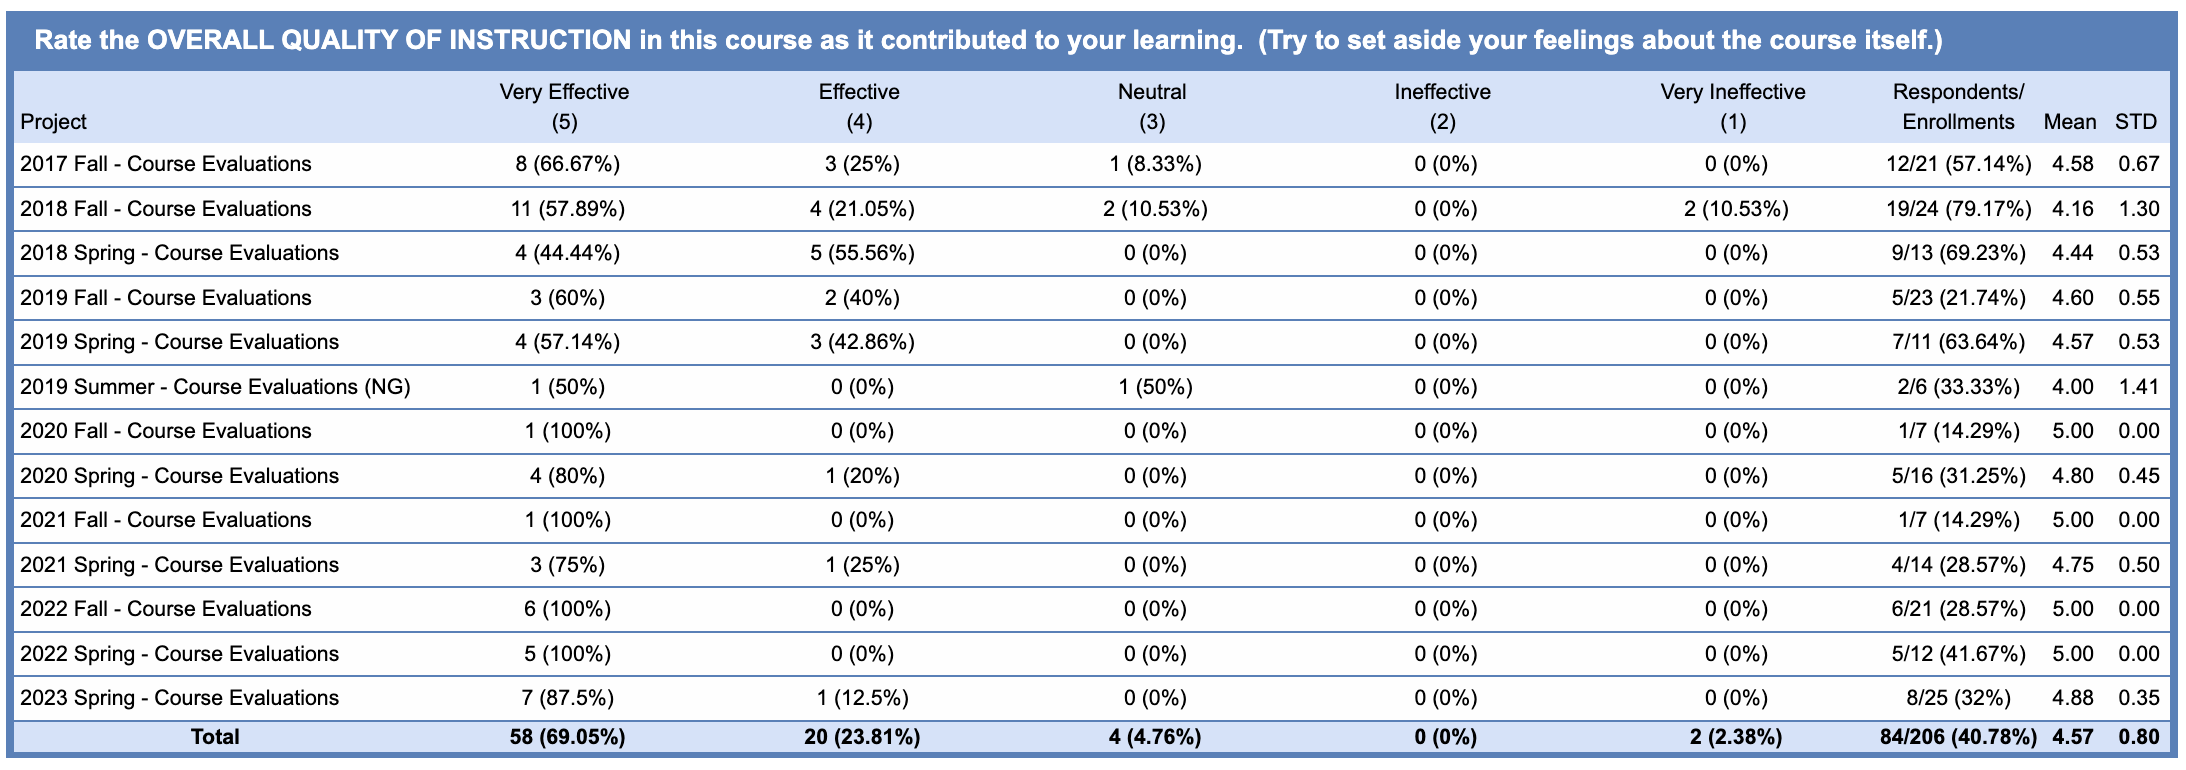
\includegraphics[width=\textwidth]{img/avgteachingevals.png}
\end{table}

\subsubsection*{Comments from Spring 2023 Information Visualization class}
The following are the complete comments from the students submitting evaluations for the Spring 2023 Information Visualization class.

\textit{9 - What did you find most valuable about this course and instructor?}
{\fontfamily{cmss}\selectfont
\begin{tablist}
\item \tab{}I think the concept of understanding how visualization design effects each person uniquely the professor explained in great detail how to navigate these differences when presenting visualizations to end-users.
\item \tab{}The instructor incorporated student questions into his lectures, from current AND past semesters. This is really useful, as these questions are common among students, so directly tackling those issues is very helpful in the understanding of these topics.
\item \tab{}His style of teaching is very effective. He deals with students patiently and provides detailed feedback along with great potential directions.
\item \tab{}The instructor is extremely passionate about the subject, enthusiastically presents it and provides unique assignments and grading criteria's to work with. The course itself is quite interesting and showcases data and how we perceive it with visuals
\end{tablist}
}
\newpage
\textit{10 - What constructive suggestions do you have for the improvement of this course or instructor?}
{\fontfamily{cmss}\selectfont
\begin{tablist}
\item \tab{}Nothing Doctor Eskridge did an excellent job teaching this advanced topic.
\item \tab{}Maybe we could have live poster-making (Visualization) exercises in class in the future. 
\item \tab{}None
\end{tablist}
}
\subsubsection*{Comments from Fall 2022 Introduction to HCD class}
The following are the complete comments from the students submitting evaluations for the Fall 2022 Introduction to Human-Centered Design class.

\textit{9 - What did you find most valuable about this course and instructor?}
{\fontfamily{cmss}\selectfont
\begin{tablist}
\item \tab{}He is very jovial and makes the class interesting. I found the most valuable aspect of this course to be the instructor's jovial attitude. He makes the learning experience enjoyable and makes it more enjoyable to learn the material. He teaches the material in a way that not only helps me understand the material but also makes learning the material fun. He also assigns homework that is relevant to the material that is covered in the class, which helps to reinforce the concepts learned during the lectures. His teaching style is also very helpful as he uses real-world examples when explaining the concepts, which makes the material seem more relevant and easier to apply in real-life scenarios. Overall, I find his course extremely valuable as it gives me a much better understanding of the cybersecurity industry and how to be successful in this field.
\item \tab{}The conversations between professor and students was very helpful in keeping the class engaging but more time is needed. 
\item \tab{}AMAZING TEACHER
\item \tab{}Talking about the course, This course helped me to gain enough knowledge about human centered design, Dr. Eskridge is a torch barrier. He has well designed the course and his explanation was awesome.
\end{tablist}
}
\textit{10 - What constructive suggestions do you have for the improvement of this course or instructor?}
{\fontfamily{cmss}\selectfont
\begin{tablist}
\item \tab{}Possible longer class
\end{tablist}
}
\begin{table}\caption{Independent Study Courses Taught}
\label{indep}
\center
\begin{tabular}{| l | c | c | c |}
Semester & Student & Title & Evaluations \\ \hline
Fall 2023 & Ruchir Gupta & Human-centered design of wearable technology &  n.a. \\
Fall 2021 & Lauren McNair & Safety-critical systems & No \\
Spring 2021 & Andrew Biron & Ideation, prototyping and additive manufacturing & No \\
Spring 2021 & Elizabeth Reme & Human-automation teamwork & No \\
Spring 2021 & Kazuhiko Momose & Safe and effective human spaceflight & No \\
Fall 2020 & Maria Sagastume & Human-centered design of biomedical devices & No \\
\end{tabular}
\end{table}

\begin{table}\caption{Capstone Courses Supervised}
\label{capstone}
\center
\begin{tabular}{| l | c | p{2in} | c |}
Semester & Student & Title & Major  \\ \hline
Fall 2019 & Jonathan T. Checchi  & IoCSpector – Triage Automation for Indicators of Compromise & CYB \\
Spring 2019 & Christopher Garner &  Identification of Malicious URL’s using Data Mining & CYB\\
Fall 2018 & Robert Moore & Visualization of Network Status and Security Events & CYB \\
Spring 2018 & Gregory Coulter & A review of network intrusion detection systems through visualization & CYB \\
\end{tabular}
\end{table}

\begin{table}\caption{Senior Design Courses Supervised}
\label{srdesign}
\center
\begin{tabular}{| l | p{2in} | c | p{2in} |}
Semester & Topic & Enroll  & Results \\ \hline
Fall 2023 & Ambient Artificial Intelligence  & 3 & \\
Fall 2023 & Compositional Control of Autonomous Vehicles & 3 &  \\
Spring 2021 & Image Snippets & 2 & commercial support, Worked with Google on Competition problem \\
Spring 2021 & Real-time plume detection and mapping & 3 & commercial support \\
Fall 2020 & Fly VR & 2 & \\
Spring 2020 & The Music Assistant & 3 & \\
Spring 2019 & Generating Enhanced Augmented Reality Surveillance (GEARS) & 4 & commercial support \\
Fall 2018 & Enhanced Pilot Learning Interface System & 4 & assisted HCD PhD student \\
Fall 2017 & Simple Segmentation of Small Networks & 4 & Best Computer Science Project \\
\end{tabular}
\end{table}

%Provide a list of graduate students supervised. List separately Ph.D. and master’s students. Give names, dissertation/thesis titles, dates of study and current employment, if known. If any postdoctoral fellows have been supervised, list names. name of fellowship or source of support and dates. Provide a statement concerning participation on graduate student committees or include in the list above, but clearly identify whom you supervised (primary thesis/dissertation advisor) and for whom you were a committee member.

%%%--------------------
\newpage
    \subsection*{Doctoral Advisor (graduates in bold)}

    \begin{itemize}
        \item \textbf{2022 Vijayanth Tummala, Advancing Human-Agent Teamwork, CS PhD, Assistant Professor, Embry-Riddle Aeronautical University, Daytona Beach, FL}
        \item \textbf{2021 Troy Ricardo Weekes, Flow Choice Architecture: Cognitive Augmentation of Knowledge Workers, HCD PhD, Research Associate L3Harris Institute for Assured Information, Melbourne, FL}
        \item \textit{Expected Spring 2024} Kazuhiko Momose, Compositional Human-Agent Teams, HCD PhD Candidate
        \item Ali Mohammad K Almashykhi, CS PhD
        \item Alita Regi, HCD PhD
        \item Hisham Ghunaim, HCD PhD
        \item Victor Kitmanyen, HCD PhD
        \item Warren Harrell, HCD PhD
        \item Waseem Samkari, CS PhD
    \end{itemize}

    \subsection*{Masters Advisor (graduates in bold)}

    \begin{itemize}
        \item \textbf{2022 Brad Thomas Costa, A Co-Evolutionary Approach to Test Case Generation for Safety-Critical Systems, CS MS, Directory of Engineering, Sentry View Systems, Melbourne, FL}
        \item \textbf{2020 Kleanthis Zisis Tegos, Real-Time Action Classification using Intermediate Skeletal Pose Estimation, CS MS, Software Engineer, Microsoft, Miami, FL}
        \item \textbf{2018 Daljeet Kaur Kaushal, Big Data Architectures for Deep Learning, CS MS, Software Associate, Goldman Sachs, Jersey City, New Jersey}
        \item \textbf{2018 Tyler Culp, Infrastructure-based Access Policy Enforcement using Software-Defined Networks, CS MS, Software Engineer, Maxar Technologies, Melbourne FL}
        \item Andrew Biron, TAC-IT: An Affective Computing Interface Design,  HCD MS
        \item Bianca Ebanks, HCD MS
        \item Lalith Nadipalli, HCD MS
        \item Rahul Mehta, CS MS
        \item Ruchir Gupta, HCD MS, Product Designer, Prototype Lab at Groundswell, Inc., Melbourne FL
        \item Shvanand Gujjari, HCD MS
        \item Srushti Nitin Ghadge, HCD MS
        \item Uditkumar Ajitkumar Nair, HCD MS
        

    \end{itemize}

    \subsection*{Committee Member}
    \begin{itemize}
    \item current Candice Chambers, CS PhD 
    \item current Natalie N Shah, Virtual Teams as an analog (or proxy) model for evaluating ROI of human-AI team interactions, Business PhD
    \item current Christopher Stricklan, Binary Diversity, Computer Science PhD
    \item current Kendall A Carmody, The Effect of Level of Immersion on Learning in a Virtual Maintenance Training Task, AHF PhD
    \item 2023 Eric Lawrence Demirjian, Artificial Intelligence Superteams \& Augmentation Strategies: Increasing Performance of High-Functioning Virtual Team Members Via Human Machine Teaming Enhancements, Business PhD
    \item 2022 Kendall A Carmody, The Effect of Level of Immersion on Learning in a Virtual Maintenance Training Task, AHF MS External
    \item 2021 Haoruo Fu, Assessment of the Skeletonization and Motion Monitoring System for the Security Efficiency of the United States Airports, Applied Aviation Safety MS
    \item 2021 James Riswick-Estelle, Algorithms for Algorithms: Teaching Problem-Solving in Computer Science, ABA OBM MS External
    \item 2020 Mary Catherine (Kay) Michel, A Bio-inspired Classification System for Cyber-Physical-Human Identity Resolution, CS PhD
    \item 2019 Seyed Mohammad Mahdi Seyednezhad, A Network-Driven Approach for Characterizing Emoji Usage in Social Media, CS PhD
    \item 2019 Sharon Sue Chinoy, Human-Centered Enterprise Resource Maintenance Management, HCD PhD
    \item 2019 Milton Stafford, Applying Formal Methods for Integrating Advanced Algorithms in Safety Critical Systems, CS MS
    \item 2018 Fitzroy Nembhard, A Recommender System for Improving Program Security Through Source Code Mining and Knowledge Extraction, CS PhD
    \item 2018 Ondrej Doule, Adaptive Spaceship Cockpit Architecture, HCD PhD    
    \item 2018 Timothy A Davis, Illegitimate Tasks and Employee Silence: A Moderated Mediation Model, IOP MS External
    \item 2018 Dhanish Mehta, On the Automation of Cyber Experimentation, CS MS
    \item 2018 Ed Mathews, Non-thesis, Meteorology MS
    \item 2018 Caleb Ryberg, Non-thesis, Meteorology MS
    \item 2017 Samir Mammadov, High Fidelity Adaptive Cyber Emulation, IACyber MS
    \item 2016 Punica Bhardwaj, Soteria: A Persuasive eSecurity Assistant, IACyber MS
    \item 2015 Evan Lawrence Stoner, A Foundation for Cyber Experimentation CS MS

    \end{itemize}


\subsubsection*{Teaching Role and Success}

I view my role as a teacher as one of providing frameworks for students to learn.  To do this, I introduce the topic, then provide the scaffolding needed for students to understand the key elements of the topic and how those elements interact with others.  This replaces what would have been a list of facts with a way to understand those facts and apply them in practice.   My priority in class is to convey the material in a way that students can apprehend the power in the concepts and determine how they can be used and also improved.  I also stress in my classes that the projects that we undertake are not simply for a class grade, but can serve other purposes for them as well: the project might address a part of their thesis or dissertation, or address a key interest they have.  In all cases, I stress that the level of quality that is expected equivalent to what is expected in a conference publication and I also encourage them to work with me after the class has ended to publish the work.    This approach has resulted in several publications with students.\\

I strive to learn new teaching techniques through blogs, the Chronicle of Higher Education, and books such as Lang's \textit{Small Teaching}.   Drawing from the human-centered design methodology, each class is a prototype where I experiment with different strategies of ordering, organizing, and presenting the material.    Each semester, I updated the examples used and evidence provided. 

My strengths as a teacher are the enthusiasm that I bring to the course and attempt to convey to the students.  I run most of my classes as extended discussions and encourage students to participate with questions, anecdotes and extreme positions that are easy for students to disagree with.    I believe that students also have this view of my teaching, as evidenced by the student comments in previous section on teaching.

My weaknesses as a teacher are mainly organizational.  I am very wiling to spend extra time during class to exploit a good discussion, but this can cause a shift in the syllabus that needs to be communicated and adjusted in the LMS.  Early in my teaching, I received negative feedback from some students on the time it took to grade assignments.  I've since made adjustments to the course schedule and my own weekly schedule to ensure that assignments are graded within the week. 

%
% The candidate should provide a statement summarizing his/her interpretation of his/her teaching role and success in teaching at Florida Tech. The statement should present a picture of yourself as a teacher describing, where appropriate, teaching practices in areas such as:
% \begin{enumerate}
% \item the setting and communicating of course goals;
% \item overall course organization;
% \item class preparation and methods used;
% \item use of supplementary materials such as audiovisual aids, library, laboratory or field experiences;
% \item grading your student work; and
% \item your availability to students having difficulty with course materials or wishing further discussion of course topics.
% \end{enumerate}

% Where appropriate, comment on:

% \begin{enumerate}
% \item the method(s) you use to evaluate your teaching;
% \item what you regard as your main strengths as a teacher;
% \item what you regard as areas in which you need improvement as a teacher;
% \item what you are doing to improve upon these goals;
% \item course innovations or development; and
% \item any other item(s) relating to teaching effectiveness
% \item What evidence do you have that your students have the same picture of you?

% \end{enumerate}

\subsection*{Academic Advising}

Dr. Eskridge  typically advises 15-20 undergraduate CS students per semester, approximately 19 MS students in HCD, CYB, and CS, and approximately 8 Ph.D. students from CS and HCD.

\subsection*{Research and Scholarly Activities}
% The term "research" is used in its broad sense of intellectual inquiry. Essentially, the term "research" is used interchangeably with the term "scholarly activities."

% Review briefly the highlights of your research contributions. Emphasize specific contributions to knowledge, but do not become overly technical.

My research is focused on how people interact with technology to improve their performance broadly scoped.  For some applications, improved performance means faster reaction times.  For other applications, improved performance means less stress and more time in a flow state.   Performance improvement happens in three ways:  moving from cognition to perception (creating visualizations that make selecting the right action effortless), enhancing cognition (creating agents that work as teammates and provide decision support), and responding to operator state (having automation measure the cognitive and emotional state of the operator and responding accordingly). 

% Review your current and future research plans.

My near-term research plans include:

\begin{enumerate}
\item Extending our work with human-agent teams to additional domains and to complete the development of trust models for different types of teams. 
\item Extending our work in human-agent teams from cybersecurity to include space, industry, and health-care.
\item Developing reasoning technologies that will assist operators in their tasks
\end{enumerate}

% Review your research support history and future plans.

%------ Research 
%List in reverse chronological order externally funded grants and contracts. Include for each the sponsoring agency or company, dates and period of support, number of students supported and amounts funded. Give a separate or contiguous list of projects internally funded or unfunded.

Dr. Eskridge has been the principal investigator (PI) on approximately \$300K of external funding at Florida Tech.  He participated in several projects as Technical Lead amounting to \$2,368,830 in the last three years. He has also played a substantial role supporting a number of other projects at the L3Harris Institute for Assured Information as Key Personnel (KP) or Collaborator (C).  The list of projects is shown in  Table ~\ref{funding}.  

I believe that collaboration is key to having a vibrant research organization. I have always been willing to participate on projects with other PIs if the work in those projects further my own research goals and permit me to direct graduate student involvement.  Similarly, I am also happy to serve as Co-PI with junior faculty to assist them in their research goals.  My commitment to collaboration is not just within the institute or department, but extends to other Colleges in the university, evidenced by my partnership with the Bisk College of Business on TETRA. 


\begin{table}[ht!]
  \caption{Externally Funded or Pending Contracts (submitted proposals in italics)}
  \label{funding}
    \centering
    \begin{tabular}{|l|l|l|l|l|l|}
    \hline
        Agency & Role & Amount & Title & GS & Duration \\ \hline
        \textit{DARPA*} & \textit{PI} & \textit{\$849,289} & \textit{CISOC} & \textit{4} & \textit{1/24-1/26} \\
        DOTE & KP & \$160,000 & TETRA & 1 &9/23-2/24 \\
        UCLA & PI & \$5,740.00 & Diverse Intelligences  & 1 & 1/22-10/22 \\ 
        FAA & PI & \$160,000.00 & Human Input Systems for CST  & 3 & 6/21-8/22 \\ 
        AFRL/BBN & PI & \$134,878.00 & LEAP & 0 & 6/21-9/22 \\ 
        AFRL/BBN & TL & \$300,000.00 & LWAP-BART & 3 & 7/20-7/22 \\ 
        AFRL/BBN & TL & \$150,000.00 & WAND  & 2 &  5/19-5/20 \\ 
        DHS    & TL     & \$1,618,212.00 & FDCE   & 3  & 9/18 - 9/21 \\ 
        AFRL/BBN & C     & \$212,500.00 & DICE & 1 &8/17-7/19 \\ 
        DoD    & TL     & \$485,841.00 & MTO & 2 & 11/17-11/18 \\ 
        DHS    & KP     & \$1,285,246.00 & FC2  & 4 &  7/14-12/18 \\ 
        AFRL   & TL     & \$1,000,000.00 & SAWD-2 &3 & 1/17-9/18 \\ 
        AFRL   & KP     & \$1,311,881.00 & SAWD-1 & 3 & 3/15-1/17 \\ 
        AFRL/BBN & KP     & \$870,000.00 & CHOPD & 1 &  3/15-9/18 \\ 
        AFRL/BBN & TL     & \$399,000.00 & BART & 2 & 4/16-11/18 \\ 
        AFRL/BBN & TL     & \$150,000.00 & InDEED & 3  &4/16-4/18 \\ 
        DHS/IAI & C     & \$522,000.00 & SDNA & 2 & 9/16-9/18 \\ 
        Securboration & C     & \$150,000.00 & JCAUSE & 0&  1/17-1/19 \\ 
        AFRL   & KP     & \$1,933,000.00 & SBC2  & 3 & 2/13-11/16 \\ 
        Rockwell Collins&KP  &\$100,000.00& APM & 1 & 3/14-9/15\\ \hline
As PI & & 		\$300,618.00 & \\
As PI/TL last 3 years & & 		\$2,368,830.00 & \\
As PI/TL & & \$6,336,671.00 & \\
Total involvement  &&		\$10,948,298.00 & \\ \hline
    \end{tabular}
\end{table}

%----
\subsection*{Research and Scholarly Activities}

A full list of publications can be found in the publications section of the Resume.  Table~\ref{tab:pubs} shows the number of publications of each type over my career, and my h-index and number of citations.  It is typical for researchers in computer science to focus on conference publications because the field is changing so quickly.  Table~\ref{confh5} shows the h5-index and h5-median scores of a number of the conferences I have published in.  These values reflect the five year average h-index for the conference.  Where additional ranking data was available, I have added that, too.  The h5-index and h5-median for journals I have published in are shown in Table~\ref{journalh5}.  This table also includes the impact factor for each journal. 

Recently, one of our papers was awarded ``Applied Human Factors And Ergonomics 2023 and its Affiliated Conferences AHFE 2023 \textbf{Best Paper Award for Human Factors in Transportation (AVI)}''
% List publications and contributions. List these publications in the following order or in chronological order indicating in the margin the appropriate category. Copies of some or all publications should be included in "Supporting Documentation for Research and Related Activities" (Appendix AIII). If too bulky, part or all of this section may be separated from the main dossier.

% \begin{enumerate}
% \item Books and monographs
% \item Articles in refereed journals and books
% \item Articles in non-refereed journals or books
% \item Articles in refereed journals or books in press
% \item Articles in non-refereed journals or books in press
% \item Articles in refereed journals or books submitted
% \item Articles in non-refereed journals or books submitted
% \item Conference presentations and whether the entire paper and/or the abstract only was reviewed.
% \item Published technical reports.
% \item Other publications such as course manuals, guidebooks, etc.
% \item List and describe briefly any disclosures of inventions or resulting patents.
% \end{enumerate}


\begin{table}[]
\caption{Publication Count and Citations
}
\label{tab:pubs}
\center
\begin{tabular}{llcl}
\hline
\multicolumn{1}{|l|}{\multirow{2}{*}{Publication Type}} & \multicolumn{1}{c|}{\multirow{2}{*}{Count}} & \multicolumn{2}{c|}{google Scholar}                                                 \\ \cline{3-4} 
\multicolumn{1}{|l|}{}                                  & \multicolumn{1}{c|}{}                       & \multicolumn{1}{c|}{h-index}             & \multicolumn{1}{l|}{i-index}             \\ \hline
\multicolumn{1}{|l|}{Conference Proceedings}            & \multicolumn{1}{l|}{74}                     & \multicolumn{1}{c|}{\multirow{5}{*}{19}} & \multicolumn{1}{l|}{\multirow{5}{*}{28}} \\ \cline{1-2}
\multicolumn{1}{|l|}{Journal}                           & \multicolumn{1}{l|}{11}                     & \multicolumn{1}{c|}{}                    & \multicolumn{1}{l|}{}                    \\ \cline{1-2}
\multicolumn{1}{|l|}{Book Chapter}                      & \multicolumn{1}{l|}{5}                      & \multicolumn{1}{c|}{}                    & \multicolumn{1}{l|}{}                    \\ \cline{1-2}
\multicolumn{1}{|l|}{Edited Book}                       & \multicolumn{1}{l|}{1}                      & \multicolumn{1}{c|}{}                    & \multicolumn{1}{l|}{}                    \\ \cline{1-2}
\multicolumn{1}{|l|}{Patents}                           & \multicolumn{1}{l|}{14}                     & \multicolumn{1}{c|}{}                    & \multicolumn{1}{l|}{}                    \\ \hline
\multicolumn{1}{r}{Total Publications}                  & 104                                         & \multicolumn{1}{l}{}                     &                                          \\
\multicolumn{1}{r}{Total Citations}                     & 2354                                        & \multicolumn{1}{l}{}                     &                                         
\end{tabular}
\end{table}

% Provide a brief statement regarding the impact of these publications in the field of research. A recommended indicator of scholarly impact would be a review of the candidate’s publications citation rate. Include a statement of the ranking of these journals in the candidate’s research field.

\begin{table}
\caption{Conference Ranking by h5-index}
\label{confh5}
\center
\begin{tabular}{|p{3in}|c|c|c|c|}
Pub & h5-index & h5-median & Rank  & Google Scholar \\ \hline
Computer Human Interaction (CHI)& 122 & 174  & top 7.46\% of 804 & \#1 in HCI\\ 
HCI International& 38 & 55 & & \#18 in HCI\\
IEEE Symposium Series on Computational Intelligence& 29 & 49 &  & \\
IEEE International Symposium on Robot and Human Interactive Communication & 28 & 31 & & \\
International Conference on Applied Human Factors and Ergonomics & 23 & 28 &  & \\
International Conference on Agents and Artificial Intelligence (ICAART)& 20 & 31 & 31.73\% of 750 & \\
Proceedings IEEE SoutheastCon & 20 & 26 & & \\
IEEE International Symposium on Parallel and Distributed Processing with Applications & 19 & 26 & & \\
International Midwest Symposium on Circuits and Systems (MWSCAS) & 18 & 23 & & \\
NASA Formal Methods & 16 & 25 & & \\
Case-Based Reasoning and Development (ICCBR)& 15& 18 & top 27.48\% of 1492 & \\
IEEE International Conference on Human-Machine Systems& 11& 14 & & \\
International Syposium on Methodologies for Intelligent Systems (ISMIS) & 9 & 15 & & \\
\end{tabular}
\end{table}


\begin{table}
\caption{Journal Ranking by h5-index}
\label{journalh5}
\center
\begin{tabular}{|p{4in}|c|c|c|c|}
Pub & h5-index & h5-median  & IF\\ \hline
  IEEE Systems Journal& 77 & 106 & 4.4  \\
Journal of Experimental \& Theoretical Artificial Intelligence & 29 & 41 & 2.2  \\
Analog Integrated Circuits and Signal Processing & 27 & 34  & 1.77 \\
KI-Künstliche Intelligenz & 26 & 37  & 2.88 \\
Metaphor and Symbol& 19 & 23  & 1.38 \\
Journal of Information and Knowledge Management (JIKM)& 3 & 6  & 1.2 \\
American Intelligence Journal& 3 & 4  & -- \\
\end{tabular}
\end{table}

  

% List invited lectures of special note during the last three years.
\subsection*{Invited Talks and Patents}

To avoid repetition, these sections are shown in the résumé.  

  % \nocite{*}
  %   \begin{refcontext}[sorting=ydnt]{}
  %   \printbibliography[keyword={INVITED}, title={Invited Talks},env=myPublicationListYearStyle, type=book]
  %   \printbibliography[keyword={INVITED-LOCAL}, title={Campus Talks},env=myPublicationListYearStyle, type=book]
  %   \printbibliography[title={Patents},env=myPublicationListYearStyle, type=misc]    \end{refcontext}


% The candidate should provide a brief statement on his/her interpretation of the role and success of his/her scholarly activities and discuss plans for future creative work and research. Comment on how you have developed yourself professionally in your discipline since your last promotion/appointment to Florida Tech.

\newpage
\subsection*{Service Activities}
To avoid repetition, these sections are shown in the résumé.

\subsection*{Documentation of Professional Practice Activities}
%This section should be used for candidates to report professional activities that do not fit conveniently under the above headings. Such activities might include consulting, professional clinical practice, short-course development, etc.

%List organizations, approximate level of effort and period of consulting. To the extent propriety permits, describe the consulting effort and the work product(s); e.g., reports, drawings, software, new test procedures, \documentclass{article}
%List short-course offerings by title, date, duration, location and approximate attendees. Describe your role as course developer and/or presenter.
I have consulted with three different companies since I came to Florida Tech.   A six month contract with Modus Operandi of Melbourne, FL supported an SBIR contract they had to develop cyber operator visualizations for their workflow.  I conducted a cognitive task analysis for the project to ensure the design of the visualization would meet the needs of the operator.  Sentry View Systems contracted me for two months to assist them with a project to test a lightweight, mobile ground system for detecting small UAVs.  I wrote flightpath creation software that allowed them to simulate drone paths using hardware-in-the-loop testing.  

I have a continuing relationship with HyLighter, LLC of Tallahassee, FL.  My work there has focused on product and market development for HyLighter's eponymous product.   This includes feature testing, prototyping, and experimentation.  

\vspace{1in}

\subsection*{Résumé} \newpage
%The résumé should be current and detailed. If the résumé provides the information requested in the above sections, that section can reference the résumé. For example, it is not necessary to list publications in "Research and Scholarly Activities" (Section III) if the data requested is clearly given in the résumé. 


\newpage
\newpage
    % display your name as the document title
    \namefont{\myname}

    % affiliation and contact info blocks
    \vspace{1em}
    \begin{minipage}[t]{0.700\textwidth}
        % current primary affiliation, left-aligned
        Department of Computer Science and Human-Centered Design \\
        L3Harris Institute of Assured Information \\
        Florida Institute of Technology
    \end{minipage}
    \begin{minipage}[t]{0.295\textwidth}
        % contact info details, right-aligned
        \flushright{}
        \href{mailto:teskridge@fit.edu}{teskridge@fit.edu} \\
        +1 321 674 7455 \\
        \href{https://thomaseskridge.com}{https://thomaseskridge.com}
    \end{minipage}


    \section*{Education}

    \begin{tablist}

        \item[Ph.D.] \tab{}Philosophy: Philosophy, Computers, and Cognitive Science \\Binghamton University, 2012. \\
                            Dissertation: Continuous Flow Analogical Reasoning
        \item[M.S.]  \tab{}Computer Science \\Southern Illinois University, Carbondale,  1987. \\
			 Thesis: Analogical Problem Solving
        \item[B.S.]  \tab{}Computer Science \\Southern Illinois University, Carbondale,  1986.


    \end{tablist}



    \section*{Appointments}

    \begin{tablist}

        \item[2015--]   \tab{}Florida Institute of Technology \\
                              Associate Professor, Department of Computer Science and Human-Centered Design and\\
                              L3Harris Institute for Assured Information

        \item[2014--15]   \tab{}Florida Institute of Technology \\
                              Research Associate Professor, L3Harris Institute for Assured Information
                              
    \end{tablist}

    \section*{Professional Experience}

    \begin{tablist}

        \item[2012--15]   \tab{}Institute for Human and Machine Cognition\\
                              Research Scientist, Human-centered computing and visualization

        \item[2001--12]   \tab{}Institute for Human and Machine Cognition\\
                              Research Associate, Human-centered computing and visualization
                              
        \item[1992--01]\tab{}Intelligent Reasoning Systems, Inc.\\
                              Founder, Chief Scientist, Automated Visual Inspection
 
         \item[1990--92]\tab{}Computing Research Laboratory, New Mexico State University\\
                              Computing Specialist II, Model-based Reasoning
                              
        \item[1989--90]\tab{}Lockheed Missiles and Space Corporation\\
                              Senior Scientific Programmer, Spatial Computing and Organizational Movement
    \end{tablist}

    \section*{Research Areas}

    \begin{itemize}

        \item Human-centered, human-aware artificial intelligence
        \item Visualization for explainability and human performance enhancement
        \item Human-automation teamwork

    \end{itemize}



\section*{Publications}\label{cvpubs}
    \nocite{*}
    \begin{refcontext}[sorting=ydnt]{}

    \printbibliography[title={Conferences},env=myPublicationListYearStyle, type=inproceedings,heading=subbibliography]
    \printbibliography[keyword={PEER}, title={Journals},env=myPublicationListYearStyle, type=article,heading=subbibliography]
    \printbibliography[keyword={WORKING}, title={Invited Journals},env=myPublicationListYearStyle, type=article,heading=subbibliography]
    \printbibliography[keyword={PUB},title={Edited Volumes},env=myPublicationListYearStyle, type=book,heading=subbibliography]
    \printbibliography[title={Book Chapters},env=myPublicationListYearStyle, type=incollection,heading=subbibliography]
    \printbibliography[title={Patents},env=myPublicationListYearStyle, type=misc,heading=subbibliography]
    \end{refcontext}

  
%    \section*{Invited Talks}

    \nocite{*}
    \begin{refcontext}[sorting=ydnt]{}
    \printbibliography[keyword={INVITED}, title={Invited Talks},env=myPublicationListYearStyle, type=book,heading=subbibliography]
    \printbibliography[keyword={INVITED-LOCAL}, title={Campus Talks},env=myPublicationListYearStyle, type=book,heading=subbibliography]
    \end{refcontext}


\newpage 
    \section*{Grants and Awards}

Grants participated in as Principal Investigator (PI), Technical Lead (TL) or Contributor (C).

\begin{table}[!ht]
    \centering
    \begin{tabular}{|l|l|l|l|l|l|}
    \hline
      Agency & Role & Amount & Title & GS & Duration \\ \hline
        \textit{DARPA*} & \textit{PI} & \textit{\$849,289} & \textit{CISOC} & \textit{4} & \textit{sub abs 1/24-1/26} \\
        DOTE & KP & \$160,000 & TETRA & 1 &9/23-2/24 \\
        UCLA & PI & \$5,740.00 & Diverse Intelligences  & 1 & 1/22-10/22 \\ 
        FAA & PI & \$160,000.00 & Human Input Systems for CST  & 3 & 6/21-8/22 \\ 
        AFRL/BBN & PI & \$134,878.00 & LEAP & 0 & 6/21-9/22 \\ 
        AFRL/BBN & TL & \$300,000.00 & LWAP-BART & 3 & 7/20-7/22 \\ 
        AFRL/BBN & TL & \$150,000.00 & WAND  & 2 &  5/19-5/20 \\ 
        DHS    & TL     & \$1,618,212.00 & FDCE   & 3  & 9/18 - 9/21 \\ 
        AFRL/BBN & C     & \$212,500.00 & DICE & 1 &8/17-7/19 \\ 
        DoD    & TL     & \$485,841.00 & MTO & 2 & 11/17-11/18 \\ 
        DHS    & KP     & \$1,285,246.00 & FC2  & 4 &  7/14-12/18 \\ 
        AFRL   & TL     & \$1,000,000.00 & SAWD-2 &3 & 1/17-9/18 \\ 
        AFRL   & KP     & \$1,311,881.00 & SAWD-1 & 3 & 3/15-1/17 \\ 
        AFRL/BBN & KP     & \$870,000.00 & CHOPD & 1 &  3/15-9/18 \\ 
        AFRL/BBN & TL     & \$399,000.00 & BART & 2 & 4/16-11/18 \\ 
        AFRL/BBN & TL     & \$150,000.00 & InDEED & 3  &4/16-4/18 \\ 
        DHS/IAI & C     & \$522,000.00 & SDNA & 2 & 9/16-9/18 \\ 
        Securboration & C     & \$150,000.00 & JCAUSE & 0&  1/17-1/19 \\ 
        AFRL   & KP     & \$1,933,000.00 & SBC2  & 3 & 2/13-11/16 \\ 
        Rockwell Collins&KP  &\$100,000.00& APM & 1 & 3/14-9/15\\ \hline
As PI & & 		\$300,618.00 & \\
As PI/TL last 3 years & & 		\$2,368,830.00 & \\
As PI/TL & & \$6,336,671.00 & \\
Total involvement  &&		\$10,948,298.00 & \\ \hline
    \end{tabular}
\end{table}

\newpage
    \section*{Conference Activity}

    \subsection*{Program Committee}
    \begin{tablist}
        \item[2023] \tab{}Senior Committee Florida Conference on Recent Advances in Robotics (FCRAR)
        \item[2020-22] \tab{}Florida Conference on Recent Advances in Robotics (FCRAR)
        \item[2022] \tab{}Association for the Advancement of Artificial Intelligence (AAAI) Conference on Artificial Intelligence
        \item[2022] \tab{}Artificial Intelligence in Education
        \item[2014-23] \tab{}International Conference on  Biologically Inspired Cognitive Architectures (BICA)
        \item[2018] \tab{}International Conference on Case-Based Reasoning (ICCBR)
        \item[2004-14] \tab{}Conferences on Concept Mapping 
        \item[2002-05] \tab{}Florida Artificial Intelligence Research Society FLAIRS Conference
        \item[1992] \tab{}Third Workshop on Battlefield Intelligence for AirLand Operations
        \item[1991] \tab{}The Second Workshop of Weather and Terrain for the Intelligence Preparation of the Battlefield
    \end{tablist}

    \subsection*{Tracks Chaired}
    \begin{tablist}
        \item[2018] \tab{}\enquote{Human-agent teamwork for cyber operations} Florida Artificial Intelligence Research Society Conference (FLAIRS-31)
    \end{tablist}

    \subsection*{Sessions Chaired}

    \begin{tablist}

        \item[2021] \tab{}\enquote{Challenges in Teaming.} CAE-R Workshop on the human element in autonomous cyber security, Melbourne, FL

    \end{tablist}

    \subsection*{Invited Panelist}
    \begin{tablist}
      \item[2023] \tab{}''The human element'', Adaptive Cyber Defense 2023, Melbourne, FL
    \end{tablist}

    \subsection*{Peer Review}

    \begin{tablist}
        \item[2012-21] \tab{}International Conference on Biologically Inspired Cognitive Architectures
        \item[2004-14] \tab{}International Conference on Concept Mapping
        \item[2020-23] \tab{}Florida Conference on Recent Advances in Robotics (FCRAR)
        \item[2022-23] \tab{}Association for the Advancement of Artificial Intelligence (AAAI) Conference on Artificial Intelligence
        \item[2018] \tab{}International Conference on Case-Based Reasoning (ICCBR)
        \item[2004-14] \tab{}Conferences on Concept Mapping 
        \item[2002-05] \tab{}Florida Artificial Intelligence Research Society FLAIRS Conference
    \end{tablist}


    \section*{Courses Taught}

    \begin{itemize}
        \item CSE5800 Interacting with Large Language Models (Created)
        \item HCD6380 Creative and Design Thinking (Created)
        \item HCD5802 Usability Engineering (Created)
        \item HCD6701 Research Methods (Created) 
        \item CYB5800 Information Visualization (Created)
        \item CSE5400 Introduction to Human-Centered Design (Created)
        \item CSE5800 Deep Learning (Created)
        \item CSE5290 Introduction to Artificial Intelligence (Created)
        \item CSE5310 Management and Processing of Big Data (Created)
        \item CYB5800 Network Security Reasoning (Created) 
        \item CYB5675 Data Mining for Cybersecurity (Created)
    \end{itemize}

    \section*{Service}

    \subsection*{Academic Journal Editorial Boards}

    \begin{itemize}
        \item \textit{Journal of Theoretical and Experimental Artificial Intelligence}  2016--
    \end{itemize}

    \subsection*{Academic Journal Peer Review}

    \begin{itemize}
        \item \textit{Journal of Theoretical and Experimental Artificial Intelligence}
        \item \textit{IEEE Transactions on Cybernetics}
        \item \textit{IEEE Transactions on Systems, Man, and Cybernetics}
        \item \textit{Sustainability}
        \item \textit{Applied Sciences}
        \item \textit{Multimodal Technologies and Interaction}
        \item \textit{Frontiers in Psychology}
        \item \textit{Electronics}
        \item \textit{Information}
        \item \textit{Biologically Inspired Cognitive Architectures (BICA) Journal}
    \end{itemize}

    \subsection*{Funding Agency Peer Review}

    \begin{itemize}

        \item National Science Foundation

    \end{itemize}

    \subsection*{Service to University}

    \begin{itemize}
        \item Served on the University Library Committee
        \item Served on the University Research Council
    \end{itemize}

    \subsection*{Service to College}

    \begin{itemize}
        \item Served as Co-Chair of the College Promotion and Tenure Committee
        \item Served on the College Promotion and Tenure Committee
        \item Served as Co-Chair of the COES Dean search committee
    \end{itemize}

    \subsection*{Service to Department}

    \begin{itemize}
        \item Redeveloped Human Centered Design Master's and Ph.D. programs
        \item Admissions for Human Centered Design Master's and Ph.D. programs
        \item Assisted in creation and development of Data Science Certificate and Degree Program
        \item Developed four of the five required HCD core classes (with support from graduate students)
        \item Developed CYB 5675  Data mining for cybersecurity course for on campus and on line use
    \end{itemize}

    \subsection*{Doctoral Advisor (graduates in bold)}

    \begin{itemize}
        \item \textbf{2022 Vijayanth Tummala, Advancing Human-Agent Teamwork, CS PhD, Assistant Professor, Embry-Riddle Aeronautical University, Daytona Beach, FL}
        \item \textbf{2021 Troy Ricardo Weekes, Flow Choice Architecture: Cognitive Augmentation of Knowledge Workers, HCD PhD, Research Associate L3Harris Institute for Assured Information, Melbourne, FL}
        \item \textit{expected Spring 2024} Kazuhiko Momose, Compositional Human-Agent Teams, HCD PhD Candidate
        \item current Ali Mohammad K Almashykhi, CS PhD
        \item current Alita Regi, HCD PhD
        \item current Hisham Ghunaim, HCD PhD
        \item current Victor Kitmanyen, HCD PhD
        \item current Warren Harrell, HCD PhD
        \item current Waseem Samkari, CS PhD
    \end{itemize}

    \subsection*{Masters Advisor (graduates in bold)}

    \begin{itemize}
        \item \textbf{2022 Brad Thomas Costa, A Co-Evolutionary Approach to Test Case Generation for Safety-Critical Systems, CS MS, Directory of Engineering, Sentry View Systems, Melbourne, FL}
        \item \textbf{2020 Kleanthis Zisis Tegos, Real-Time Action Classification using Intermediate Skeletal Pose Estimation, CS MS, Software Engineer, Microsoft, Miami, FL}
        \item \textbf{2018 Daljeet Kaur Kaushal, Big Data Architectures for Deep Learning, CS MS, Software Associate, Goldman Sachs, Jersey City, New Jersey}
        \item \textbf{2018 Tyler Culp, Infrastructure-based Access Policy Enforcement using Software-Defined Networks, CS MS, Software Engineer, Maxar Technologies, Melbourne FL}
        \item current Andrew Biron, HCD MS
        \item current Bianca Ebanks, HCD MS
        \item current Lalith Nadipalli, HCD MS
        \item current Rahul Mehta, CS MS
        \item Ruchir Gupta, HCD MS, Product Designer, Prototype Lab at Groundswell, Inc., Melbourne FL
        \item current Shivanand Gujjari, HCD MS
        \item current Srushti Nitin Ghadge, HCD MS
        \item current Uditkumar Ajitkumar Nair, HCD MS
    \end{itemize}

    \subsection*{Committee}
    \begin{itemize}
    \item current Natalie N Shah, Virtual Teams as an analog (or proxy) model for evaluating ROI of human-AI team interactions, Business PhD
    \item current Christopher Stricklan, Binary Diversity, Computer Science PhD
    \item current Candice Chambers, Computer Science PhD
    \item  2023 Eric Lawrence Demirjian, Artificial Intelligence Superteams \& Augmentation Strategies: Increasing Performance of High-Functioning Virtual Team Members Via Human Machine Teaming Enhancements, Business PhD
    \item 2022 Kendall A Carmody, The Effect of Level of Immersion on Learning in a Virtual Maintenance Training Task, AHF MS External
    \item 2021 Haoruo Fu, Assessment of the Skeletonization and Motion Monitoring System for the Security Efficiency of the United States Airports, Applied Aviation Safety MS
    \item 2021 James Riswick-Estelle, Algorithms for Algorithms: Teaching Problem-Solving in Computer Science, ABA OBM MS External
    \item 2020 Mary Catherine (Kay) Michel, A Bio-inspired Classification System for Cyber-Physical-Human Identity Resolution, CS PhD
    \item 2019 Seyed Mohammad Mahdi Seyednezhad, A Network-Driven Approach for Characterizing Emoji Usage in Social Media, CS PhD
    \item 2019 Sharon Sue Chinoy, Human-Centered Enterprise Resource Maintenance Management, HCD PhD
    \item 2019 Milton Stafford, Applying Formal Methods for Integrating Advanced Algorithms in Safety Critical Systems, CS MS
    \item 2018 Fitzroy Nembhard, A Recommender System for Improving Program Security Through Source Code Mining and Knowledge Extraction, CS PhD
    \item 2018 Ondrej Doule, Adaptive Spaceship Cockpit Architecture, HCD PhD    
    \item 2018 Timothy A Davis, Illegitimate Tasks and Employee Silence: A Moderated Mediation Model, IOP MS External
    \item 2018 Dhanish Mehta, On the Automation of Cyber Experimentation, CS MS
    \item 2018 Ed Mathews, Non-thesis, Meteorology MS
    \item 2018 Caleb Ryberg, Non-thesis, Meteorology MS
    \item 2017 Samir Mammadov, High Fidelity Adaptive Cyber Emulation, IACyber MS
    \item 2016 Punica Bhardwaj, Soteria: A Persuasive eSecurity Assistant, IACyber MS
    \item 2015 Evan Lawrence Stoner, A Foundation for Cyber Experimentation CS MS

    \end{itemize}

    \section*{Memberships}

    \begin{itemize}

        \item Association for the Advancement of Artificial Intelligence (AAAI)
        \item American Association for the Advancement of Science (AAAS)
        \item Sigma Xi
        \item Cognitive Science Society
        \item Institute of Electrical and Electronics Engineers (IEEE)
    \end{itemize}



    \section*{Consulting}

    \begin{tablist}
        \item[2020--  ] \tab{}HyLighter, LLC, Tallahassee, FL
        \item[2021--21] \tab{}Sentry View Systems, Melbourne, FL
        \item[2016--17] \tab{}Modus Operandi, Melbourne, FL
    \end{tablist}

\subsection*{Supporting Documentation for Teaching and Related Activities}
Course evaluations are included in the file ``Eskridge-course-evaluations.pdf''

\subsection*{Supporting Documentation for Research and Related Activities}
A collection of the first page of many of my papers and patents are included in the file ``Eskridge-titlepages.pdf''.  A selection of representative papers is included in the file ``Eskridge-FivePapers.zip''.  Access to all full papers is available at \url{https://www.thomaseskridge.com}.

\end{document}

    % display today's date as Month Year after a vertical space below the end of the text
    \begin{center}
        \vfill
        Updated \monthyeardate\today
    \end{center}



% Items in this appendix would normally include copies of papers, but could also include copies of proposal abstracts, letters of research awards, or letters of notification of honors, such as outstanding paper awards. If the list of research activities called for in "Research and Scholarly Activities" (Section III) is extensive, it could be included here and referred to in that section.

% \subsection*{Supporting Documentation for Service Activities}
% Items included here could be letters of commendation, copies of service reports authored by the candidate, or more detailed descriptions of service than is possible in "Service Activities" (Section IV).

% \subsection*{Supporting Documentation for Professional Practice}
% Items included here might include notification of professional registration, letters of commendation for consulting or clinical practice, or syllabi and manuals developed for short-courses, workshop or conferences.

% \subsection*{Department Head Letter of Nomination}
% This appendix will contain two important letters:

% \begin{itemize}
% \item A brief letter from the candidate addressed to the department head/program chair that states "This letter certifies that I have reviewed my dossier and that the entries and substantiation thereof are accurate."
% \item A letter from the department head/program chair nominating the candidate for promotion. The letter should state the degree of support for the nomination in the department/program. For promotion to full professor, identifying the support of the department’s/program’s full professors is important. Copies of the faculty member’s annual goal/performance evaluations for the past three years could be included in this appendix.
% \end{itemize}

% \subsection*{Letters of Recommendation from Outside Reviewers}
% Include a brief statement of the credentials of each person from whom letters have been solicited. It is expected that for promotion to full (associate) professor at least five (three) letters will be solicited. Include what aspect of the candidate’s performance the referee is competent to judge and why. Include all letters received. These letters should be added to the dossier by the department head/program chair after the candidate has made his/her final review of the dossier to afford the recommender’s confidentiality.

% The academic unit head should write all requests for evaluations. The candidate should not solicit these letters although s/he may suggest names of references. The letters of request should clearly state what kind of an evaluation is being sought (the factors to be evaluated, the rank for which the person is being recommended and other pertinent information). Wherever reasonable, one or both of the following questions should be asked. From what you know of this person, would you recommend him/her for promotion at your institution?

% Where does the candidate rank among his/her peers? As a courtesy to those being asked to write letters, a current copy of the candidate’s résumé should be sent.

